	%% ------------------------------------------------------------------------- %%
\chapter{Introdução}
\label{cap:introducao}

O processo de implantação de um software vai do momento de aquisição do software até o momento em que o software se encontra em execução~\cite{DEPL2006}. Processos totalmente automatizados são importantes na implantação de sistemas \cite{Humble2011Continuous}. No entanto, muitas organizações ainda realizam a implantação de seus sistemas conforme descrita por Dolstra et al. \cite{Dolstra2005Configuration}: um processo manual, moroso, propenso a erros e não reprodutível. Ainda segundo esses autores, o problema se agrava na implantação de sistemas distribuídos, pois o esforço de implantação cresce com a quantidade de nós do sistema. Em cenários de grande escala, um processo de implantação manual se torna inviável. Esses cenários vem sendo discutidos academicamente e ainda não há soluções consolidadas \cite{Valerie2011FutureInternet}.

Pesquisadores acreditam que a arquitetura da Internet atual não comportaria todos os requisitos dos serviços do futuro, o que leva a criação de uma nova arquitetura, denominada Internet do Futuro \cite{Zahariadis2011FutureInternet}. Na Internet do Futuro, espera-se a existência de complexas composições de bilhões de serviços web, formando coreografias de milhões de recursos, pessoas e coisas \cite{Valerie2011FutureInternet}. No entanto, o desenvolvimento de colaborações entre serviços trazem desafios para a formulação de mecanismos que funcionem, escalem e que sejam eficientemente implementados em um ambiente distribuído de grande escala \cite{Steen2011VeryLarge}.

Sistemas distribuídos estão migrando para ambientes de nuvem, onde são compostos e mantidos de modo descentralizado por várias organizações \cite{Steen2011VeryLarge}. A computação em nuvem possibilita o acesso a um conjunto compartilhado de recursos computacionais que podem ser providos rapidamente \cite{Nist2011Cloud}. A gerência programática desses recursos virtualizados favorece a criação de processos totalmente automatizado para a implantação de sistemas \cite{Humble2011Continuous}.   

Steen~\cite{Steen2011VeryLarge} destaca que um sistema distribuído de grande escala normalmente não é fornecido por uma única organização e que, portanto, ninguém é responsável por ``todo o sistema''. Essa necessidade de distribuição dificulta a execução de atividades que precisam ser coordenadas entre as organizações, pois nenhuma das partes detém o controle sobre toda a infraestrutura. O aspecto interorganizacional normalmente implica também na heterogeneidade tecnológica, pois partes da aplicação mantidas por organizações diferentes costumam ser construídas com tecnologias diferentes, como por exemplo Java ou .NET. Quando essas partes do sistema precisam se comunicar diretamente surge a necessidade de uma comunicação interoperável, o que é possibilitado por serviços web. 

Serviços web possibilitam a comunicação interoperável entre máquinas pela rede \cite{W3C2004WS}. Um exemplo é a consulta a um serviço do correio para verificação de preços e prazos de diferentes opções de entrega. A existência de um serviço web que forneça essa funcionalidade possibilita que uma loja, por exemplo, selecione dinamicamente a opção de entrega mais vantajosa de acordo com os requisitos de seus clientes. Serviços também são compostos para implementar processos de negócios sofisticados \cite{Papazoglou2007State}. Nessa situação, serviços web são diretamente ligados uns aos outros. Se existem supermercados que oferecem serviços web para consulta de preço e compra de produtos, pode-se elaborar um processo de negócio em que um consumidor faça uma busca automatizada em diferentes supermercados procurando o menor preço para a sua compra. A coordenação de um processo de negócio ocorre de forma centralizada ou distribuída. No caso centralizado, denominado orquestração \cite{Nanda2004Decentralizing}, há um orquestrador que determina como os outros serviços web envolvidos no processo de negócio devem se relacionar. No caso distribuído, denominado coreografia \cite{Barker2009Choreographing}, cada serviço sabe como e com quais parceiros deve interagir. 

Para compor uma orquestração ou coreografia, é preciso que os serviços identifiquem a localização (URIs) de suas dependências. Em um processo de implantação na nuvem, não se pode fazer suposições sobre os endereços IPs dos serviços antes da implantação, o que requer um modelo de configuração flexível, considerando a natureza dinâmica da nuvem \cite{Amazon2012Practices}. Dessa forma, o processo de implantação de coreografias requer algum mecanismo dinâmico de troca de endereços entre os serviços participantes. 

Embora exista uma diversidade de técnicas para aumentar a disponibilidade de aplicações e serviços, quando um sistema interage com outro independente, normalmente pertencente a outra organização, é preciso sempre considerar uma possível indisponibilidade do sistema invocado na outra organização. Em sistemas de grande escala, tais falhas ocorrem com maior frequência. Por isso, esses sistemas precisam ser projetados para que continuem a funcionar na presença de falhas de seus componentes, mesmo que para isso tenham que continuar operando com funcionalidades reduzidas \cite{Hamilton2007InternetScale,  Helland2009Quicksand}.

Considerando os desafios já colocados, a questão que guia esta pesquisa é ``\emph{como realizar a implantação automatizada de coreografias de serviços web de grande escala em ambientes distribuídos de computação em nuvem.}'' O objetivo desta dissertação é solucionar a questão colocada por meio da arquitetura de um arcabouço que dê suporte à implantação automatizada de coreografias de serviços web em ambientes de computação em nuvem. 

Em nosso trabalho, as coreografias de serviços web se enquadram no seguinte contexto:

\begin{itemize}
\item Uma coreografia possui serviços web de diferentes organizações.
\item Os serviços web de uma mesma coreografia podem ser implantados em diferentes infraestruturas, pertencentes a diferentes organizações.
\item As organizações utilizarão infraestruturas de computação em nuvem.
\item Diferentes organizações podem utilizar diferentes tecnologias de nuvem.
\end{itemize}

O arcabouço proposto deve ainda contemplar os seguintes requisitos:

\begin{itemize}
\item Com a ajuda do arcabouço, o processo de implantação das coreografias deve ser totalmente automatizado.
\item Deve-se privilegiar construções tolerantes a falha, ou seja, se um componente do sistema falha, o sistema inteiro continua a responder, mesmo que com funcionalidade reduzida.
\item Considerando magnitudes de milhares de serviços em centenas de nós, o tempo de implantação deve ser escalável, ou seja, conforme se aumente a quantidade de serviços a serem implantados e a quantidade de nós disponíveis, o tempo de implantação deve permanecer idealmente constante. 
\item A implantação de uma coreografia com centenas de serviços deve ocorrer com tempo na ordem de poucos minutos.
\end{itemize}

Nossa solução consiste no desenvolvimento do CHOReOS Enactment Engine, um arcabouço que fornece uma Plataforma como Serviço (PaaS) para a execução de processos automatizados de implantação de coreografias de serviços web. Para realizar a implantação das coreografias em um ambiente de nuvem, o Enactment Engine utiliza Infraestrutura como um Serviço (IaaS) de outros provedores de computação de nuvem. A arquitetura de nossa solução em termos das camadas da computação em nuvem pode ser observada na Figura~\ref{fig:camadas_nuvem}.

\begin{figure}[!h]
  \centering
  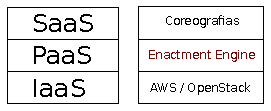
\includegraphics[width=.50\textwidth]{camadas.pdf} 
  \caption{Camadas da computação em nuvem associadas à nossa solução.}
  \label{fig:camadas_nuvem} 
\end{figure}

Listaremos agora as fases do processo de implantação de um sistema~\cite{DEPL2006}, para logo em seguida explicar a quais fases nosso arcabouço oferece suporte.

\begin{description}
\item [Instalação:] a organização adquire os componentes e os disponibilizam em sua infraestrutura interna. Em sistemas orientados a serviços, normalmente a organização que desenvolve o componente é a mesma que realiza a implantação, fazendo dessa etapa uma mera questão de gerar os pacotes a partir do código-fonte e torná-los acessíveis dentro da organização.
\item [Configuração:] arquivos de configuração são editados para personalizar comportamentos funcionais dos componentes de acordo com as necessidades da organização; um exemplo típico é a configuração de uma conexão a um banco de dados. Essa fase dificilmente pode ser automatizada.
\item [Planejamento:] mapeamento de como os componentes serão distribuídos pela infraestrutura alvo, que contem os nós onde os componentes são instalados.
\item [Preparação:] procedimentos no ambiente de implantação, normalmente envolvendo configurações do sistema operacional e instalação de middlewares.
\item [Inicialização:] transferências dos componentes para os nós onde serão executados, ligação entre os componentes de uma composição e execução dos componentes.
\end{description}

O \ee\ se preocupa principalmente com a automação das fases de preparação e de inicialização dos serviços. Em nosso processo assumimos que as fases de instalação e configuração já estão realizadas. Sobre o planejamento, o \ee\ oferece suporte ao planejamento dinâmico sobre como os serviços serão distribuídos pelos nós de uma nuvem, mas cabe ao operador executar parte do planejamento que é determinar em que nuvem os componentes serão implantados.

Os aspectos de grande escala considerados pelo arcabouço são a 1) automatização do processo de implantação, 2) consideração da natureza dinâmica do ambiente de computação em nuvem, 3) o tratamento adequado de erros de componentes de terceiros, 4) um projeto de API assíncrona e idempotente, e 5) pontos de extensão para lidar com a heterogeneidade tecnológica.

Ainda como validação da aplicação do arcabouço em um cenário de grande escala, o mesmo será avaliado pela escalabilidade do tempo de implantação, variando-se a quantidade de serviços a serem implantados e a quantidade de nós disponíveis no ambiente computação em nuvem. O objetivo é que um aumento proporcional na carga -- serviços a serem implantados -- e nos recursos disponíveis -- máquinas virtuais -- não altere significativamente o tempo de implantação.

Esta pesquisa é feita no contexto e com financiamento dos projetos CHOReOS e Baile, que estudam a aplicação de coreografias de serviços em ambientes de grande escala. O projeto CHOReOS\footnote{http://www.choreos.eu}, financiado pela Comissão Europeia e composto por diversas instituições acadêmicas e industriais da Europa conjuntamente com o IME-USP, introduz um processo dinâmico e centrado no usuário para o desenvolvimento de coreografias em um ambiente de escala ultra grande, no qual milhares de serviços são compostos e coordenados por um middleware distribuído. O projeto Baile\footnote{http://ccsl.ime.usp.br/baile/}, uma parceria entre IME-USP e HP Labs, estuda a solução de problemas para o desenvolvimento de coreografias, como a adoção de Desenvolvimento Guiado por Testes (TDD) no contexto de coreografias e o suporte da Computação em Nuvem à implantação de coreografias.

Este trabalho se organiza da seguinte forma: as fundamentações teóricas sobre composição de serviços e computação de grande escala são apresentadas, respectivamente, no Capítulo~\ref{cap:servicos} e no Capítulo~\ref{cap:escala}. Os trabalhos relacionados, sobre implantação de sistemas, são apresentados no Capítulo~\ref{cap:relacionados}. No Capítulo~\ref{cap:solucao} apresentamos nossa solução proposta. Por fim, temos nosso plano de trabalho no Capítulo~\ref{cap:cronograma}. 


%% ------------------------------------------------------------------------- %%
%\section{Considerações Preliminares}
%\label{sec:consideracoes_preliminares}
%
%\section{Objetivos}
%\label{sec:objetivo}
%
%\section{Contribuições}
%\label{sec:contribucoes}
%
%\section{Organização do Trabalho}
%\label{sec:organizacao_trabalho}
%
